\section{Sistemi Quantistici Aperti}
Fino a questo punto le considerazioni che sono state fatte non includevano in alcun modo la considerazione dell'interazione dell'ambiente con il sistema stesso. Di per se la considerazione dell'ambiente viene fatta solo "concettualmente" per vedere l'utilità di alcuni operatori (come la traccia parziale). In questa sezione si pone l'obiettivo di spiegare come andare ad affrontare la considerazione dell'ambiente. I metodi principalmente presentati sono due. Uno basato sulla \textbf{Quantum Operatorion Formalism} ed uno basato sul \textbf{Master Equation Formalism}.

\subsection{Quantum operations Formalism}
Il quantum operation formalism è uno strumento che permette di andare a valutare il sistema a valle di un opearzione che avviene in modo Black Box. Per comprendere al meglio tale differenza si considera un esempio preso dal libro \cite{nielsen2010}. Quando si va ad effettuare una singola operazione unitaria su di un sistema single qubit quello che si ottiene è un sistema del tipo visualizzabile nella figura [\ref{img:single-system}]

\begin{figure}[H]
\centering
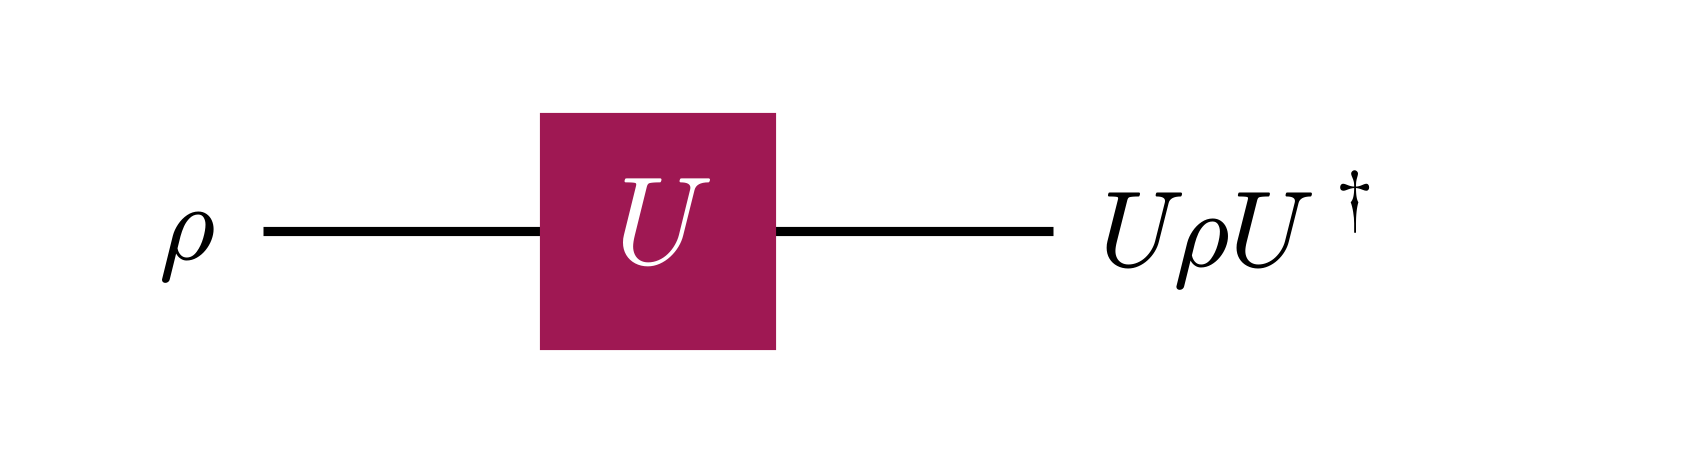
\includegraphics[width=.7\textwidth]{fig/Chapter-3/sistema_chiuso.png}
\caption{Sistema Chiuso}\label{img:single-system}
\end{figure}

Quindi in tale sistema l'operazione U agisce solamente sul nostro sistema di interesse senza tenere conto dell'ambiente. Mentre nel caso della Quantum Operation si va a considerare anche un contributo \(\rho_{env}\) che è legato all'ambiente. Nella figure [\ref{img:double-system}] è mostrato quello che si intende. Precisamente, in tale immagine si considera che i due sistemi prima dell'operazione non siano in alcun modo interagenti.

\begin{figure}[H]
\centering
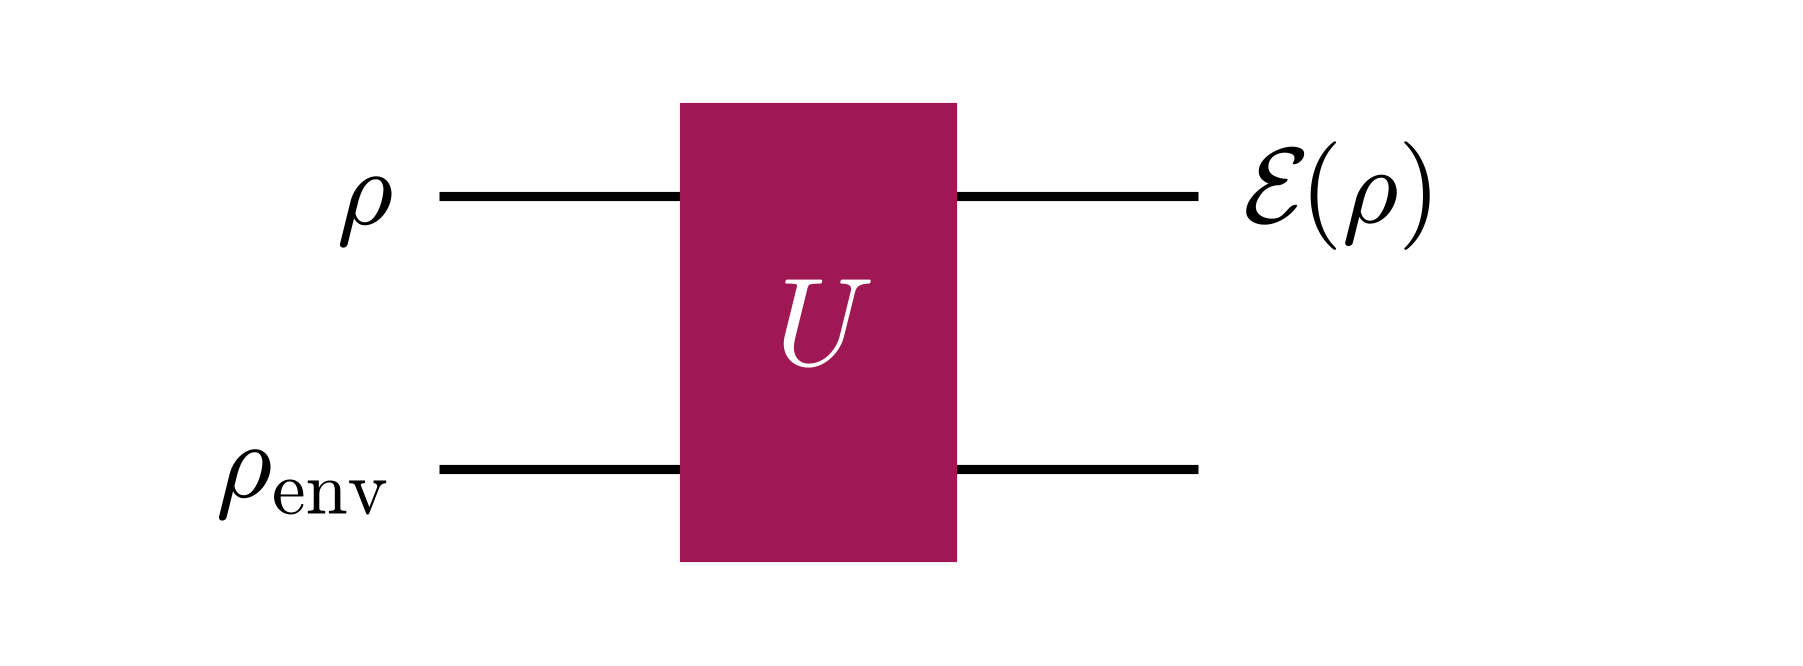
\includegraphics[width=.7\textwidth]{fig/Chapter-3/sistema_aperto.png}
\caption{Open Quantum System}\label{img:double-system}
\end{figure}

Quindi sarà possibile dire che \(\rho'\) (Matrice di densità associata allo stato successivo all'operazione) è calcolabile rispetto a \(\rho\) (Matrice di densità associata allo stato prima dell'operazione). Ottenendo:

\begin{gather*}
    \rho' = \varepsilon(\rho)
\end{gather*}

Dove la \(\varepsilon\) è la quantum operation. Tale operazione può generalizzare sia operazioni unitarie su un sistema chiuso (caso in cui l'operazione U non vada a generare delle iterazioni con il sistema considerato), definendo operazioni del tipo \(\varepsilon(\rho)=U \rho U^\dagger\), sia di descrivere vere e proprie operazioni di misura \(\varepsilon(\rho) = M_m \rho M_m^\dagger \). Le quantum operations, quindi, sono possibili tutte le operazioni fisicamente possibili.

I principali metodi utilizzati per lo studio delle quantum operation sono:
\begin{itemize}
    \item \textbf{Sistema accoppiato con l'ambiente}: Sì va a studiare la dinamica del sistema in base al suo accoppiamento con l'ambiente. Un pò come succede nel caso classico. Non è molto conveniente matematicamente nonostante la sua grande vicinanza alla realtà
    
    \item \textbf{Rappresentazione Somma-operatore}: Sistema che considera le stesse identiche cose del primo metodo, con la differenza che cerca di sopperire all'inconvenienza matematica con la rappresentazione somma operatore. Tale metodologia è molto astratta ma è utile per i calcoli e per i lavori teorici

    \item \textbf{Assiomi fisicamente motivati}: Metodologia che utilizza degli assiomi che vengono definiti sulla base di risultati provenienti dalla meccanica quantistica. Ci si aspetta che tali assiomi siano soddisfatti da una funzione dinamica nella meccanica quantistica
\end{itemize}

\subsubsection{Sistema Accoppiato con l'ambiente}
Un primo modo di studiar eil nostro sistema è quello di andare a considerare l'ambiente parte di un sistema chiuso. Quindi il sistema chiuso da considerare è quello del mio sistema effettivo più il contributo portato dall'ambiente. Come visto nell'immagine [\ref{img:double-system}]. Supponendo di avere come stato del nostro sistema \(\rho\), e di processarlo mediante un'operazione \(U\) che va ad accoppiarlo con l'ambiente, si ottiene che l'operazione \(\varepsilon(\rho)\) non è relativa ad un'operazione unitaria (dispersione negli stati con l'ambiente). Supponendo che prima dell'operazione il sistema sia in uno stato del tipo \(\rho \otimes \rho_{env}\), allora dopo l'operazione sarà possibile ricondursi allo stato del sistema principale mediante l'utilizzo della traccia parziale:

\begin{gather*}
    \varepsilon(\rho) = tr_{env}\left[U (\rho \otimes \rho_{env})U^\dagger\right]
\end{gather*}

Tale operazione, nel caso in cui l'operatore \(U\) non crei interazione (entanglement) tra il sistema e l'ambiente permette di poter scrivere il sistema come \(\rho \otimes \rho_{env}\) il che rende più facile il calcolo della traccia parziale e quindi di poter definire l'operazione come:
\begin{gather*}
    \varepsilon(\rho) = \tilde{U} \rho \tilde{U^\dagger}
\end{gather*}
dove \(\tilde{U}\) è definito come lamparte di \(U\) che agisce sul primo sistema in maniera isolata.
Però nelle situazioni reali questa cosa accade molto raramente. Solitamente il sistema è entanglato con l'ambiente e quindi il calcolo della traccia parziale dev'essere effettuato mediante la sua specifica definizione. E quindi andando a studiare tutta la dinamica del sistema principale + l'ambiente (che è un operazione cdi per se molto complessa). Lo stato dell'ambiente non è mai determinato ed è impossibile da controllare.

\subsubsection{Rappresentazione somma-operatore}
La rappresentazione somma operatore è unatipologia di considerazione che ci permette di andare a valutare il sistema in una maniera più generale. Andando a scrivere la \(\varepsilon(\rho)\) come:
\begin{gather*}
    \varepsilon(\rho) = \sum_k \bra{e_k} U (\rho \otimes \ket{e_0}\bra{e_0}) U^\dagger \ket{e_k}
\end{gather*}

Che è la definizione estesa della traccia parziale andando a considerare l'insieme dei vettori \(\ket{e_k}\) una base ortonormale per lo spazio di stato dell'ambiente, si ottiene che:
\begin{align*}
    \varepsilon(\rho) &= \sum_k \bra{e_k} U (\rho \otimes \ket{e_0}\bra{e_0}) U^\dagger \ket{e_k}\\
    &=\sum_k \bra{e_k} U \left[(I \otimes \ket{e_0}) \rho (I \otimes \bra{e_0})\right] U^\dagger \ket{e_k}\\
    &= \sum_k \bra{e_k}U\ket{e_0} \rho \bra{e_0} U^\dagger \ket{e_k}
\end{align*}
Dove nell'utlimo passaggio vi è un \textbf{abuso di notazione} che permette di estendere l'operazione \(\ket{e_k} = (I \otimes \ket{e_k})\), questo perchè nella prima equazione \(\ket{e_k}\) ha dimensione pari a quelle del sottosistema facente riferimento all'ambiente (quindi dimensione ridotta), mentre nel secondo caso è l'estensione di tale base per il sistema ridotto al sistema complessivo. La \(I\) sta ad indicare che sul sistema principale non vi sono operazioni, mentre sul secondo sistema sì. 
Fatta questa definizione, ponendo \(E_k = \bra{e_k} U \ket{e_0}\), si ottiene che:
\begin{gather*}
    \varepsilon(\rho) = \sum_k E_k \rho E_k^\dagger
\end{gather*}

Questa è la definizione della rappresentazione somma operatore del sistema descritto. Gli operatori \(\{E_k\}\) sono noti come elementi dell'operazion per l'operazione quantistica \(\varepsilon(\rho)\). Per la trace-preserving quantum operations (operazioni quantistiche che non variano la traccia della matirce di densità, quindi non cambiano le "probabilità" associate ai singoli autostati) vi è bisogno di rispettare la seguente proprietà:
\begin{gather*}
    \sum_k E_k^\dagger E_k = I
\end{gather*}

Questo è visualizzabile considerando uno stato puro per cui:
\begin{gather*}
    1 = tr(\varepsilon(\rho)) = tr\left(\sum_k E_k \rho E_k^\dagger\right) = tr\left(\sum_k E_k^\dagger E_k \rho\right)
\end{gather*}

Da cui la proprietà precerdente. Nel caso delle non-trace-preserving quantum operations invece, tale somma non sarà identicamente l'identità \(I\). Ma sarà definita come:
\begin{gather*}
    \sum_k E_k^\dagger E_k \le I
\end{gather*}

Quindi la rappresentazione somma operatore permette di poter considerare la dinamica del sistema senza andare ad esplicirare le proprietà dell'ambiente.

\subsubsection{Assiomi fisicamente motivati}
Nel caso degli assiomi si vanno a porre degli assiomi che sono fisicamente motivati e collegati alla dinamica del sistema fisico stesso. Gli assiomi che vengono posti sono:
\begin{itemize}
    \item \textbf{A1}: La probabilità che \(\varepsilon(\rho)\) occorra è definita come \(0 \le tr(\varepsilon(\rho)) \le 1 \)
    
    \item \textbf{A2}: \(\varepsilon\) è una funzione lineare convessa sulla matrice di densità, per cui:
    \begin{gather*}
        \varepsilon\left(\sum_k p_k \rho_k\right) = \sum_k p_k \varepsilon(\rho_k)
    \end{gather*}

    \item \textbf{A3}: \(\varepsilon\) è una funzione completamente positiva per qualunque \(\rho\)
\end{itemize}

Dati tali assiomi è dimostrabile che una funzione \(\varepsilon\) che soddisfi tutti gli assiomi è definibile se e solo se:
\begin{gather*}
    \varepsilon(\rho) = \sum_k E_k \rho E_k^\dagger \\ \sum_k E_k^\dagger E_k \le I
\end{gather*}

La rappresentazione somma operatore non è unica, quindi si avrà che:
\begin{gather*}
    \varepsilon(\rho) = \sum_k E_k \rho E_k^\dagger = \sum_k F_k \rho F_k^\dagger\\
    F_k = \sum_l U_{kl} E_l
\end{gather*}
Dove \(U\) è una matrice unitaria (\(U^{-1} = U^\dagger\)).
ù

\subsection{Master Equation}
Oltre allo strumento della quantum operation è possibile andare a studiare il sistema anche mediante l'utilizzo della master equation. Più precisamente, il \textbf{master equation formalism} è un formalismo matematico che va a studiare l'andamento di \(\rho\) tramite la master equation. Tale formalismo è meno generale rispetto a quello adottato nella quantum operations formalism. Difatti un processo quantistico descritto mediante la rappresentazione somma operatore non è detto sia riscrivibile mediante la master equation. La master equation ha come vantaggio quello di poter andare a valutare i disturbi ed i loro comportamenti sullo stato generale del sistema. Si riporta la lindblad form della master equation:
\begin{gather*}
    \frac{d}{dt}\rho(t) = -\frac{i}{\hbar}\left[H_s, \rho(t)\right] + \sum_k \left(L_k \rho(t)L_k^\dagger - \frac{1}{2}\{L_k^\dagger L_k, \rho(t)\}\right)
\end{gather*}

Dove la notazione \([A,B] = AB - BA\) e \(\{A,B\} = AB + BA\). Mentre gli elementi dell'equazione sono:
\begin{itemize}
    \item \(\hbar\): Costante di Planck
    \item \(H_s\): Hamiltoniano del sistema, è un operatore hermitiano, per sistemi chiusi, la sua conoscenza vuol dire conoscere l'evoluzione della dinamica del sistema (anche in questo caso non dipendente dal tempo)
    
    \item \(\{L_k\}\): Operatori di Lindblad, rappresentano l'accoppiamento del sistema con l'ambiente
    
    \item \(d^2-1\): Numero di operatori di Lindblad indipendenti associati ad un sistema di \(d\) qubit. Racchiudono tutte le possibili dissipazioni.
    
    \item Per un sistema a singolo qubit si può definire \(L_k = \sqrt{\gamma_k}\Omega_k, k \in {x,y,z}\). Dove il \(\gamma_k\) mi permette di capire quanto il mio sistema sia accoppiato con l'ambiente rispetto alla specifica matrice di Pauli (Tasso di decoerenza per lo specifico canale \(k\))
\end{itemize}

\subsubsection{Z-Noise}
Definita l'equazione è anche possibile andare a notare, componente per componente, come agisce il rumore sulle singole componenti. Considerando un rumore presente solo sull'asse \(z\) si definisce \(L_z = \sqrt{\gamma_z}\Omega_z\) e \(\frac{H_s}{\hbar} = \frac{\Omega}{2}\Omega_z\). Sostituendo nella master equation si ottiene:

\begin{gather*}
    \frac{d}{dt}\rho(t) = -i\left[\frac{\Omega}{2}\Omega_z, \rho(t)\right] + L_z \rho(t) L_z^\dagger - \frac{1}{2}\{L_z^\dagger L_z, \rho(t)\}
\end{gather*}

Proseguendo nei calcoli si ottiene che:
\begin{gather*}
\frac{d}{dt}\rho(t) = -\frac{i \Omega}{2}
\left[\begin{smallmatrix}
0 & 2 \rho^{01}(t)\\
-2\rho^{10}(t) & 0
\end{smallmatrix}\right] +
\gamma_z
\left[\begin{smallmatrix}
0 & -2 \rho^{01}(t)\\
-2\rho^{10}(t) & 0
\end{smallmatrix}\right] = 
\left[\begin{smallmatrix}
0 & -(i\Omega + 2 \gamma_z)\rho^{01}(t)\\
(i\Omega-2 \gamma_z)\rho^{10}(t) & 0
\end{smallmatrix}\right]
\end{gather*}

Gli elementi sulla diagonale principale sono nulli data la loro costanza nel tempo (le probabilità non cambiano). Quindi \(\rho^{jj}(t) = \rho^{jj}(0), \forall t, j=0,1\). Andando a risolvere le disequazioni si ottiene che:
\begin{gather*}
    \rho^{01}(t) = \rho^{01}(0)e^{-(i\Omega + 2\gamma_z)t}\\
    \rho^{10}(t) = \rho^{10}(0)e^{-(-i\Omega + 2 \gamma_z)t}= (\rho^{01}(t))^*
\end{gather*}

Quindi un qubit arbitrario accumula una fase \(\Omega t\) rispetto alla differenza di energia tra \(\ket{0}\) e \(\ket{1}\). Conoscendo \(\Omega\), l'evoluzione di fase può essere compensata mediante una gate di shift di fase \(R_{\Omega t}\) che va ad agire sul sistema ponendo il seguente risultato:
\begin{gather*}
    \rho(t) = R_{\Omega t} \rho R_{\Omega t}^\dagger = \left[\begin{smallmatrix}
        \rho^{00}(0) & \rho^{01}(0)e^{-2 \gamma_z t}\\
        \rho^{10}(0)e^{-2 \gamma_z t} & \rho^{11}(0)
    \end{smallmatrix}\right]\\
    R_{\Omega t} = \left[\begin{smallmatrix}
        1 & 0\\
        0 & e^{-i \Omega t}
    \end{smallmatrix}\right]
\end{gather*}

Andando ad esplicitare la \(\rho\) nella forma \(\rho = \frac{1}{2}(I + r_x \Omega_x + r_y \Omega_y + r_z \Omega_z)\), si ottiene che:
\begin{align*}
    r_x(t) &= r_x(0)e^{-2 \gamma_z t}\\
    r_y(t) &= r_y(0)e^{-2 \gamma_z t}\\
    r_z(t) &= r_z(0)
\end{align*}

Che ci spiega come il sistema ruota attorno solo all'asse \(z\), guardando la sfera di bloch. Andando riducendosi attorno all'asse \(z\). 

\subsubsection{X-Noise}
Come nel caso dello Z-Noise, si considera il rumore sulla rotazione lungo X, si va a definire quindi \(L_x = \sqrt{\gamma_x}\sigma_x\) con \(\frac{H_s}{\hbar} = \frac{\Omega}{2}\sigma_z\). Una volta impostati questi valori si prosegue nella soluzione dell'equazione:
\begin{gather*}
\frac{d}{dt}\rho(t) = -i \left[\frac{\Omega}{2}\sigma_z,\rho(t)\right] + L_x \rho(t) L_x^\dagger - \frac{1}{2}\{L_x^\dagger L_x, \rho(t)\}
\end{gather*}

Andando a risolvere tale equazione si otterrà:
\begin{gather*}
    \rho(t) = 
    \frac{1}{2}
    \left[\begin{smallmatrix}
    \rho^{00}(t)(0)(1 + e^{-2 \gamma_x t}) + \rho^{11}(0)(1 - e^{-2 \gamma_x t}) & \rho^{01}(0)(1+e^{-2 \gamma_x t}) + \rho^{10}(0)(1 - e^{-2 \gamma_x t})\\
    \rho^{10}(0)(1+e^{-2 \gamma_x t}) + \rho^{01}(0) (1 - e^{-2 \gamma_x t}) & \rho^{11}(0)(1+e^{-2 \gamma_x t}) + \rho^{00}(0)(1 - e^{-2 \gamma_x t})
    \end{smallmatrix}\right]
\end{gather*}

Andando ad esplicitare il sistema come \(\rho = \frac{1}{2}(I + r_x \sigma_x + r_y \sigma_y + r_z \sigma_z)\), si ottiene:
\begin{align*}
r_x(t) &= r_x(0)\\
r_y(t) &= r_y(0)e^{-2 \gamma_x t}\\
r_z(t) &= r_z(0)e^{-2 \gamma_x t}
\end{align*}

A mano a mano si entrava nella sfera di Bloch andando a convergere poi, solo alla fine, sulla sola componente \(r_x\).

\subsection{Somme}
Il rumore quantistico, quindi è moltiplicativi (agisce sul vettore di bloch per un certo valore non uguale tra tutti) andando ad intaccare in maniera non uguale tutte le coordinate del sistema, tale comportamento è stato anche descritto da chip quantistici reali.
In generale, lo Z-noise non va ad intaccare la popolazione (elementi sulla diagonale di \(\rho\)) ma va ad intaccare le coerenze (elementi fuori diagonale), mentre l'X-Noise va anche ad intaccare gli elementi sulla diagonale, portando anche a possibili Bit-Flip. L'Y-Noise (non visto), è una combinazione di ambo i rumori, quindi va ad intaccare tutto come nel caso dell'X-Noise.